\documentclass[11pt]{article}

\usepackage[utf8]{inputenc}
\usepackage[T1]{fontenc}
\usepackage{lmodern}
\usepackage[protrusion=true,expansion=true]{microtype}
\usepackage{amsmath,amssymb}
\usepackage{graphicx}
\usepackage{booktabs}
\usepackage{array}
\usepackage{longtable}
\usepackage{xcolor}
\usepackage{float}
\usepackage[margin=1in]{geometry}
\usepackage[round,authoryear]{natbib}
\usepackage[font=small,labelfont=bf,labelsep=period]{caption}
\usepackage[hidelinks]{hyperref}
\hypersetup{
  colorlinks=true,
  linkcolor={black!65!blue},
  citecolor={black!55!green},
  urlcolor={black!65!blue},
  pdftitle={A Release-Pinned and Temporally Sealed PIM1 QSAR Benchmark},
  pdfauthor={Tair Narynov}
}

\graphicspath{{figures/}}
\setlength{\parindent}{1.2em}
\setlength{\parskip}{0.15em}
\renewcommand{\arraystretch}{1.13}
\newcolumntype{L}[1]{>{\raggedright\arraybackslash}p{#1}}
\newcolumntype{R}[1]{>{\raggedleft\arraybackslash}p{#1}}

% All numerical claims below are generated directly from immutable artifacts.
% Generated by scripts/08_build_manuscript_assets.py; do not edit by hand.
\newcommand{\SnapshotActivityCount}{4,861}
\newcommand{\SnapshotAssayCount}{986}
\newcommand{\SnapshotParentCount}{3,112}
\newcommand{\BroadEligibleCount}{4,380}
\newcommand{\BroadEventCount}{3,356}
\newcommand{\BroadCompoundCount}{3,106}
\newcommand{\StrictEventCount}{1,125}
\newcommand{\StrictCompoundCount}{1,087}
\newcommand{\NoHighTailEventCount}{1,110}
\newcommand{\NoHighTailCompoundCount}{1,072}
\newcommand{\HomologousExcludedCount}{2,973}
\newcommand{\StructureFailureCount}{0}
\newcommand{\MultiEventCompoundCount}{24}
\newcommand{\DispersionHalfCount}{10}
\newcommand{\DispersionOneCount}{6}
\newcommand{\StrictAssayContextCount}{122}
\newcommand{\StrictDocumentContextCount}{102}
\newcommand{\StrictDescriptionContextCount}{89}
\newcommand{\AssayEventMedian}{3}
\newcommand{\AssayEventMinimum}{1}
\newcommand{\AssayEventMaximum}{65}
\newcommand{\LargestAssayEventPercent}{5.8}
\newcommand{\ATPDescriptionAssayCount}{34}
\newcommand{\ATPDescriptionEventCount}{365}
\newcommand{\NumericATPAssayCount}{8}
\newcommand{\NumericATPEventCount}{117}
\newcommand{\NumericATPEventPercent}{10.4}
\newcommand{\ATPMinimumMicromolar}{20}
\newcommand{\ATPMaximumMicromolar}{5000}
\newcommand{\ATPFoldRange}{250}
\newcommand{\ATPKmAssayCount}{3}
\newcommand{\SingleEventCompoundPercent}{97.8}
\newcommand{\CrossAssayCompoundCount}{18}
\newcommand{\AssayExclusiveScaffoldEventPercent}{82.2}
\newcommand{\DevelopmentAssayCount}{68}
\newcommand{\TemporalAssayCount}{48}
\newcommand{\DevelopmentDocumentCount}{62}
\newcommand{\TemporalDocumentCount}{36}
\newcommand{\AssayPartitionOverlapCount}{0}
\newcommand{\DocumentPartitionOverlapCount}{0}
\newcommand{\MatchedATPLowMicromolar}{50}
\newcommand{\MatchedATPHighMicromolar}{5000}
\newcommand{\MatchedATPLowNanomolar}{9}
\newcommand{\MatchedATPHighNanomolar}{100}
\newcommand{\MatchedATPShift}{1.046}
\newcommand{\DevelopmentCount}{803}
\newcommand{\DevelopmentScaffoldCount}{369}
\newcommand{\TemporalCount}{284}
\newcommand{\TemporalScaffoldCount}{160}
\newcommand{\NewTemporalScaffoldCount}{149}
\newcommand{\NewTemporalCompoundCount}{251}
\newcommand{\NewTemporalCompoundPercent}{88.4}
\newcommand{\SeenTemporalCompoundCount}{33}
\newcommand{\CrossCutoffMedianShift}{0.059}
\newcommand{\CrossCutoffMaximumShift}{0.706}
\newcommand{\OuterRepeatCount}{3}
\newcommand{\OuterFoldCount}{5}
\newcommand{\SelectedModelText}{Ridge (ECFP6 + RDKit2D)}
\newcommand{\DevelopmentRMSE}{0.742}
\newcommand{\BestGraphModelText}{Edge-aware GINE (graph + RDKit2D)}
\newcommand{\BestGraphRMSE}{0.893}
\newcommand{\TunedGNNBestModelText}{nested-tuned frozen CheMeleon ensemble}
\newcommand{\TunedGNNBestRMSE}{0.754}
\newcommand{\TunedGNNBestRMSESD}{0.011}
\newcommand{\TunedGNNBestDelta}{0.002}
\newcommand{\TunedGNNBestDeltaLower}{-0.038}
\newcommand{\TunedGNNBestDeltaUpper}{0.046}
\newcommand{\TunedGNNBestMeanPredictionSeedSD}{0.170}
\newcommand{\TunedGNNBestWithinRepeatSeedRMSESD}{0.009}
\newcommand{\TunedGNNCandidateBudget}{24}
\newcommand{\TunedGNNRandomDrawCount}{23}
\newcommand{\TunedGNNRerankCount}{3}
\newcommand{\TunedGNNSeedCount}{3}
\newcommand{\TunedGNNScreeningEvaluations}{1,080}
\newcommand{\TunedGNNInnerFitCount}{4,050}
\newcommand{\BestGraphDelta}{0.070}
\newcommand{\BestGraphDeltaLower}{0.029}
\newcommand{\BestGraphDeltaUpper}{0.114}
\newcommand{\RunnerUpModelText}{RBF-SVR (ECFP6 + RDKit2D)}
\newcommand{\RunnerUpRMSE}{0.744}
\newcommand{\RunnerUpDelta}{0.002}
\newcommand{\RunnerUpDeltaLower}{-0.021}
\newcommand{\RunnerUpDeltaUpper}{0.024}
\newcommand{\DescriptorAblationConclusion}{improved GINE but not the D-MPNN}
\newcommand{\GNNCheckpointCount}{60}
\newcommand{\GNNInnerEpochCount}{180}
\newcommand{\GNNInnerEpochMinimum}{1}
\newcommand{\GNNInnerEpochMaximum}{63}
\newcommand{\GNNRefitEpochCount}{60}
\newcommand{\GNNRefitEpochMinimum}{1}
\newcommand{\GNNRefitEpochMaximum}{43}
\newcommand{\GNNEpochCap}{80}
\newcommand{\GNNEpochCapHitCount}{0}
\newcommand{\ModelComparisonConclusion}{under the prespecified modest search budget, none of the four evaluated graph variants improved on the leading ECFP6-plus-descriptor models}
\newcommand{\DiscussionModelFinding}{the bounded development comparison selected a regularized ECFP6-plus-descriptor model, without establishing a general ranking of fixed and learned representations}
\newcommand{\ConclusionFinding}{the sealed temporal audit revealed cohort-level degradation and failure of the evaluated reliability diagnostics to identify high-error predictions}
\newcommand{\TemporalRMSE}{0.972}
\newcommand{\TemporalRMSELower}{0.872}
\newcommand{\TemporalRMSEUpper}{1.075}
\newcommand{\TemporalMAE}{0.750}
\newcommand{\TemporalMAELower}{0.666}
\newcommand{\TemporalMAEUpper}{0.840}
\newcommand{\TemporalRtwo}{0.470}
\newcommand{\TemporalRtwoLower}{0.311}
\newcommand{\TemporalRtwoUpper}{0.582}
\newcommand{\TemporalGeneralizationGap}{0.231}
\newcommand{\BetweenYearVariancePercent}{31.8}
\newcommand{\WithinYearCenteredRtwoAll}{0.266}
\newcommand{\LaterCohortCenteredRtwo}{-0.046}
\newcommand{\LaterCohortCenteredSpearman}{0.286}
\newcommand{\TemporalRMSETwentyNineteen}{0.795}
\newcommand{\TemporalRMSETwentyTwentyFour}{1.261}
\newcommand{\TemporalRMSEIncrease}{0.466}
\newcommand{\TemporalRMSEIncreasePercent}{58.7}
\newcommand{\TemporalRMSEIncreaseScaffoldLower}{0.190}
\newcommand{\TemporalRMSEIncreaseScaffoldUpper}{0.733}
\newcommand{\AbsoluteErrorSlopePerYear}{0.080}
\newcommand{\AbsoluteErrorSlopeScaffoldLower}{0.038}
\newcommand{\AbsoluteErrorSlopeScaffoldUpper}{0.123}
\newcommand{\DocumentClusterRMSELower}{0.787}
\newcommand{\DocumentClusterRMSEUpper}{1.150}
\newcommand{\DocumentClusterRtwoLower}{-0.007}
\newcommand{\DocumentClusterRtwoUpper}{0.682}
\newcommand{\DocumentCenteredCount}{261}
\newcommand{\DocumentCenteredGroupCount}{19}
\newcommand{\DocumentCenteredRtwo}{-0.031}
\newcommand{\DocumentCenteredSpearman}{0.303}
\newcommand{\AssayCenteredCount}{252}
\newcommand{\AssayCenteredGroupCount}{23}
\newcommand{\AssayCenteredRtwo}{-0.146}
\newcommand{\AssayCenteredSpearman}{0.240}
\newcommand{\EarlierBroadRecordCount}{4}
\newcommand{\StrictChronologySensitivityCount}{280}
\newcommand{\StrictChronologySensitivityRMSE}{0.976}
\newcommand{\StrictChronologySensitivityRtwo}{0.463}
\newcommand{\NearestNeighborGapErrorRho}{0.271}
\newcommand{\NearestNeighborGapErrorLower}{0.122}
\newcommand{\NearestNeighborGapErrorUpper}{0.411}
\newcommand{\CalibrationSlope}{0.930}
\newcommand{\CalibrationIntercept}{0.382}
\newcommand{\IntervalWidth}{2.504}
\newcommand{\IntervalFoldSpan}{319}
\newcommand{\TemporalCoveragePercent}{81.3}
\newcommand{\CoverageLowerPercent}{75.2}
\newcommand{\CoverageUpperPercent}{86.7}
\newcommand{\OutsideADCount}{154}
\newcommand{\SimilarityErrorRho}{0.042}
\newcommand{\InsideADRMSE}{0.954}
\newcommand{\OutsideADRMSE}{0.988}
\newcommand{\NewScaffoldRMSE}{0.980}
\newcommand{\SeenScaffoldRMSE}{0.914}
\newcommand{\TemporalHighTailRemoved}{7}
\newcommand{\NoHighTailTemporalRMSE}{0.968}
\newcommand{\ClassicalPythonVersion}{3.12.3}
\newcommand{\RDKitVersion}{2026.3.3}
\newcommand{\NumPyVersion}{2.5.1}
\newcommand{\PandasVersion}{3.0.3}
\newcommand{\SklearnVersion}{1.9.0}
\newcommand{\TorchVersion}{2.12.1+cpu}
\newcommand{\PyGVersion}{2.8.0}
\newcommand{\ChempropVersion}{2.2.4}


\title{\textbf{A Release-Pinned and Temporally Sealed PIM1 QSAR Benchmark}\\[3pt]
\large Temporal reliability under joint chemical, cohort, and assay-provenance shift}
\author{Tair Narynov\\[4pt]
{\normalsize Victoria College, University of Toronto, Toronto, ON, Canada}\\[2pt]
{\normalsize Correspondence: \href{mailto:t.narynov@mail.utoronto.ca}{t.narynov@mail.utoronto.ca}}\\[2pt]
{\normalsize ORCID: 0000-0000-0000-0000}}
% TODO: replace the placeholder ORCID with the author's ORCID iD.
\date{}

\begin{document}
\maketitle

\begin{abstract}
QSAR performance estimated from public bioactivity data can be distorted by
release drift, assay mixing, structure leakage, and repeated test-set use. We
created a release-pinned benchmark of human PIM1 biochemical inhibition from
ChEMBL~37. Standardization and strict assay/target filters produced
\StrictEventCount{} measurement events for \StrictCompoundCount{} compounds. An
outcome-blind count rule fixed 2018 as the cutoff, yielding \DevelopmentCount{}
development compounds and a sealed test of \TemporalCount{} compounds first
meeting the strict cohort definition in 2019--2025. Under a prespecified, modest
tuning budget, seven
fixed-representation/baseline candidates and four graph-neural-network variants
shared repeated scaffold-disjoint assignments; all selection was confined to
development data. The selected \SelectedModelText{} achieved repeated-CV RMSE
\DevelopmentRMSE{} pIC$_{50}$ and one-time temporal RMSE \TemporalRMSE{} (95\%
scaffold-cluster bootstrap CI \TemporalRMSELower{}--\TemporalRMSEUpper{}), with
pooled $R^2=\TemporalRtwo{}$. This aggregate concealed time-local degradation:
RMSE increased from \TemporalRMSETwentyNineteen{} in 2019 to
\TemporalRMSETwentyTwentyFour{} in 2024, by \TemporalRMSEIncrease{} pIC$_{50}$
(95\% scaffold-cluster CI \TemporalRMSEIncreaseScaffoldLower{}--
\TemporalRMSEIncreaseScaffoldUpper{}). However, a document-source sensitivity
interval for pooled $R^2$ widened to \DocumentClusterRtwoLower{}--
\DocumentClusterRtwoUpper{}, and after centering within documents with at least
three compounds, $R^2$ was \DocumentCenteredRtwo{} and Spearman $\rho$ was
\DocumentCenteredSpearman{}. A training-defined Tanimoto domain described structural shift
but did not identify error-prone predictions ($\rho=\SimilarityErrorRho{}$ between
absolute error and neighbor similarity). Development and temporal labels shared
no assay or document identifiers, so the observed decline represents inseparable
chemical, cohort, and assay-provenance shift. A development-derived residual
reference band was \IntervalWidth{} pIC$_{50}$ wide (approximately a
\IntervalFoldSpan{}-fold IC$_{50}$ span) and covered
\TemporalCoveragePercent{}\% of temporal cases when defined at a 90\% development
target, limiting its potency-threshold decision value. The best prespecified
graph model obtained development RMSE \BestGraphRMSE{}. A separate post hoc,
development-only nested search spanning architecture, optimization,
featurization, initialization, and a frozen pretrained CheMeleon representation
obtained best RMSE \TunedGNNBestRMSE{}, but its paired RMSE difference from
the locked Ridge reference was \TunedGNNBestDelta{} (95\% CI
\TunedGNNBestDeltaLower{} to \TunedGNNBestDeltaUpper{}); it was not allowed to
alter the already completed temporal analysis. The principal finding
is that sealed temporal evaluation revealed reliability failures obscured by
pooled performance. This retrospective biochemical-potency benchmark does not
establish prospective activity, selectivity, cellular efficacy, ADMET properties,
or therapeutic value.
\end{abstract}

\noindent\textbf{Keywords:} PIM1; QSAR; ChEMBL; temporal validation;
scaffold split; graph neural network; assay provenance; applicability domain

\section{Introduction}

The proviral integration site for Moloney murine leukemia virus (PIM) family
comprises constitutively active serine/threonine kinases PIM1, PIM2, and PIM3.
PIM signaling has been implicated in hematological and solid malignancies, making
the family a continuing target of inhibitor discovery
\citep{nawijn2011pim,tursynbay2016pim}. A ligand-based model of PIM1 biochemical
potency can support hypothesis generation, but biochemical IC$_{50}$ alone does
not establish isoform selectivity, target engagement in cells, exposure, safety,
or clinical efficacy.

PIM1 has an atypical ATP-binding hinge: Pro123 lacks the backbone amide donor
that supplies a canonical second hydrogen bond to the adenine moiety in many
kinases \citep{kumar2005pim}. More generally, under the assumptions of simple
competitive inhibition, the Cheng--Prusoff relationship makes apparent
IC$_{50}$ conditional on substrate concentration \citep{cheng1973relationship}.
Consequently, strict target and endpoint filters can reduce ambiguity in public
PIM1 data without making measurements obtained under different ATP conditions
experimentally equivalent.

Machine-learning QSAR methods can extract useful structure--activity patterns
from public databases \citep{cherkasov2014qsar}. PIM1 studies have used small
congeneric series for 3D-QSAR and ligand-based virtual screening
\citep{aouidate2018qsar,asati2017qsar}, and more recent work has combined public
bioactivity data with classification, docking, or generative design
\citep{almukadi2023combining,schneider2020virtualpim}. Yet a model comparison is only
as credible as the experiment surrounding it. Database release changes can alter
the available records; related structures can leak across random splits; model
selection can consume the purported test set; and assay or target-confidence
heterogeneity can dominate algorithmic differences.

Graph neural networks (GNNs) offer an appealing alternative to fixed molecular
fingerprints because they learn task-specific graph representations. Directed
message-passing neural networks (D-MPNNs) have reported strong molecular-property
performance \citep{yang2019analyzing}, while graph-isomorphism-derived operators
provide expressive neighborhood aggregation \citep{xu2019powerful,hu2020strategies}.
However, learned graph representations do not universally outperform carefully
tuned fixed representations, particularly for modest, noisy bioactivity datasets
\citep{deng2023systematic}. A fair PIM1 comparison therefore needs shared compound
identities, shared splits, development-only tuning, and representation ablations.

Here we construct such a benchmark. Our primary contribution is an auditable
test of temporal reliability: (i) a ChEMBL~37 snapshot with source files, release
metadata, lineage, and SHA-256 checksums; (ii) a stringent PIM1 biochemical
cohort; (iii) an outcome-blind publication-year cutoff and immutable repeated
scaffold assignments; and (iv) a one-time temporal evaluation, followed by an
explicitly labeled post hoc audit of performance within annual chemistry
cohorts. Calibration, residual-reference-band, scaffold-novelty, and similarity-domain
diagnostics test whether common reliability summaries remain informative under
that shift. A bounded comparison of classical ECFP6/descriptor methods, an
edge-aware GINE, and a Chemprop D-MPNN is secondary. The goal is not a new
learning architecture or a general ranking of representation families; it is a
defensible account of what a target-specific model can and cannot support when
chemistry and assay provenance change over time.
Because that prespecified graph arm used only one architecture per backend, we
also report a separate post hoc development-only search with nested
hyperparameter selection, repeated initialization, and a frozen pretrained
CheMeleon representation. This addition strengthens the representation
comparison without pretending that the already-opened temporal cohort is a new
confirmatory test.

\section{Results}

\subsection{Release-pinned curation reduced target ambiguity but retained multi-assay heterogeneity}

The archived ChEMBL~37 query returned \SnapshotActivityCount{} activities,
\SnapshotAssayCount{} target assays, and \SnapshotParentCount{} parent molecules
(Fig.~\ref{fig:study-design}). Broad record-level eligibility retained
\BroadEligibleCount{} records. The confirmatory cohort additionally required a
biochemical assay, BAO single-protein format, direct target relationship,
confidence score~9, and no assayed variant. It retained \StrictEventCount{}
measurement events and \StrictCompoundCount{} standardized parent compounds
(Table~\ref{tab:curation}). The largest reduction arose from excluding
\HomologousExcludedCount{} activity records linked to homologous rather than
direct single-protein targets. This restriction is consequential: ChEMBL defines
confidence score~9 as direct assignment to a single protein and score~8 as an
assignment to a homologous single protein \citep{zdrazil2024chembl}.

An explicitly post hoc audit of the pinned assay metadata found that the strict
events came from \StrictAssayContextCount{} assays in
\StrictDocumentContextCount{} documents. The median assay contributed only
\AssayEventMedian{} events (range \AssayEventMinimum{}--\AssayEventMaximum{}),
and the largest representative assay accounted for
\LargestAssayEventPercent{}\% of events. Although descriptions for
\ATPDescriptionAssayCount{} assays mentioned ATP, only
\NumericATPAssayCount{} assays---covering
\NumericATPEventCount{}/\StrictEventCount{} events
(\NumericATPEventPercent{}\%)---stated a numeric ATP concentration. The reported
values spanned \ATPMinimumMicromolar{}--\ATPMaximumMicromolar{}~$\mu$M, a
\ATPFoldRange{}-fold range (Supplementary Table~\ref{tab:assay-context}).
Moreover, \SingleEventCompoundPercent{}\% of compounds had only one eligible
event. Median aggregation therefore summarized the few repeats that
existed but could not harmonize most single measurements. This limitation is
substantive: direct comparisons across ChEMBL IC$_{50}$ sources can contain large
inter-assay discrepancies, while careful metadata curation or matched-pair
contrasts reduce but do not eliminate them
\citep{landrum2024noise,nelen2025matched}.

The exhaustive bridge search within the machine-readable numeric-ATP subset
found only one compound measured in the same document at two explicit ATP
concentrations: \MatchedATPLowNanomolar{}~nM at
\MatchedATPLowMicromolar{}~$\mu$M ATP versus
\MatchedATPHighNanomolar{}~nM at \MatchedATPHighMicromolar{}~$\mu$M ATP, a
\MatchedATPShift{}-pIC$_{50}$ decrease \citep{dakin2012pim}. This $n=1$
observation illustrates why ATP context may matter; it is not an assay-effect
estimate or a basis for post hoc correction.

Structure standardization failed for \StructureFailureCount{} queried parents.
Only \MultiEventCompoundCount{} strict compounds had multiple independent
measurement events; \DispersionHalfCount{} had a pIC$_{50}$ range above 0.5 and
\DispersionOneCount{} above 1.0. Compound labels were medians of eligible
measurement-event pIC$_{50}$ values, preserving event lineage and dispersion
fields rather than silently pooling raw rows.

\begin{table}[t]
\centering
\caption{Curation flow for the release-pinned PIM1 dataset.}
\label{tab:curation}
\small
\begin{tabular}{L{0.58\textwidth}R{0.17\textwidth}R{0.16\textwidth}}
\toprule
\textbf{Stage} & \textbf{Records/events} & \textbf{Compounds} \\
\midrule
ChEMBL~37 activity snapshot & \SnapshotActivityCount{} & \SnapshotParentCount{} \\
Broad exact human PIM1 IC$_{50}$ eligibility & \BroadEligibleCount{} & --- \\
Broad duplicate-collapsed measurement events & \BroadEventCount{} & \BroadCompoundCount{} \\
Strict direct single-protein biochemical events & \StrictEventCount{} & \StrictCompoundCount{} \\
Strict sensitivity cohort, pIC$_{50}\leq 10$ & \NoHighTailEventCount{} & \NoHighTailCompoundCount{} \\
\bottomrule
\end{tabular}
\par\vspace{3pt}\parbox{0.94\textwidth}{\footnotesize
\textit{Note.} Records are ChEMBL activity rows. Measurement events collapse only
source-equivalent duplicates using a documented signature. Compound identity is
the standardized parent InChIKey.}
\end{table}

\begin{figure}[t]
\centering
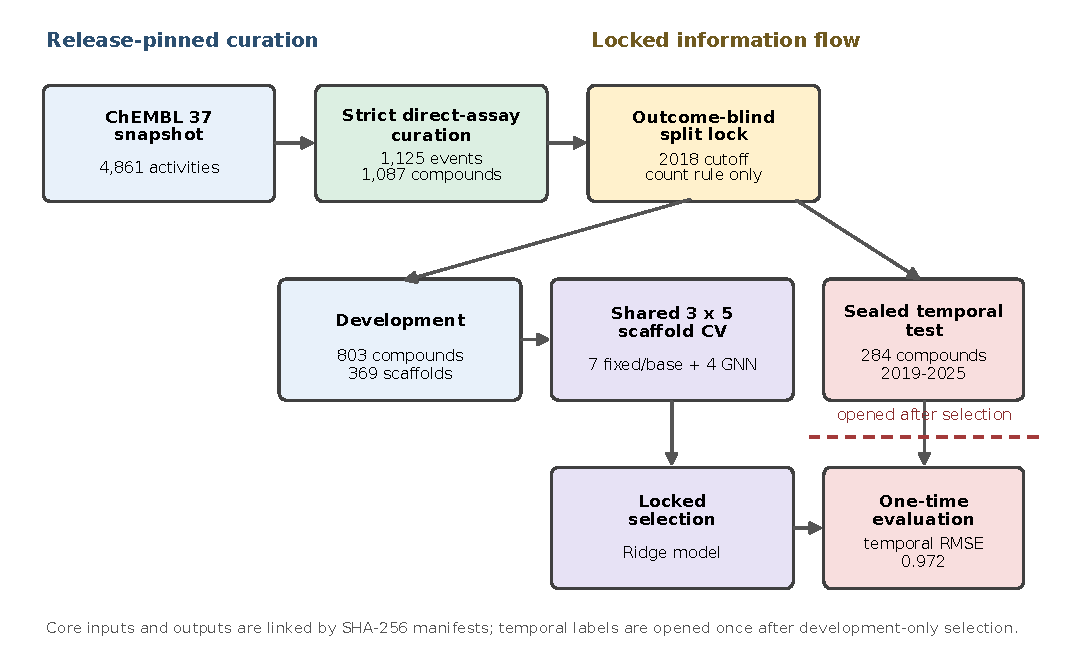
\includegraphics[width=\textwidth]{figure1_study_design.pdf}
\caption{Study design and information boundaries. The temporal cutoff was chosen
from compound and scaffold counts only. Downstream curation, split construction,
candidate fitting, hyperparameter selection, and development-only model selection
did not read temporal outcomes. The selected procedure was then refit on all
development compounds and evaluated once on the sealed temporal partition.}
\label{fig:study-design}
\end{figure}

\subsection{The count-only rule produced a demanding temporal test}

The prespecified cutoff rule selected the latest year satisfying at least 750
development compounds, 250 temporal compounds, and 100 new temporal scaffolds;
2018 was the unique latest eligible cutoff. The immutable split contains
\DevelopmentCount{} development compounds from \DevelopmentScaffoldCount{}
scaffolds and \TemporalCount{} first-seen-after-cutoff compounds from
\TemporalScaffoldCount{} scaffolds. \NewTemporalScaffoldCount{} temporal
scaffolds were absent from development, accounting for
\NewTemporalCompoundCount{} compounds (\NewTemporalCompoundPercent{}\%). Thus,
the temporal test is predominantly a joint time-and-scaffold extrapolation, while
retaining a small seen-scaffold subset for a prespecified diagnostic.

Here ``first seen'' refers specifically to an eligible event in the strict
cohort. A post hoc cross-check against the broader curated cohort found
\EarlierBroadRecordCount{} temporal identities with an earlier, non-strict
record; those earlier records failed the direct single-protein criteria. Removing
those identities left \StrictChronologySensitivityCount{} temporal compounds and
produced RMSE \StrictChronologySensitivityRMSE{} and
$R^2=\StrictChronologySensitivityRtwo{}$, so this wording correction did not alter
the substantive result.

Eleven post-2018 measurement events belonged to seven development identities.
They were quarantined in a cross-cutoff table and were not allowed to update
development labels. Across those identities, the median absolute pre/post label
shift was \CrossCutoffMedianShift{} pIC$_{50}$ and the maximum was
\CrossCutoffMaximumShift{}. This shows why aggregating all records before a
temporal split would introduce subtle future-information leakage.

\subsection{The prespecified bounded search did not reward added graph flexibility}

All candidates used the same \OuterRepeatCount{} repeated
\(\times\)\OuterFoldCount{}-fold outer assignments. Each outer validation
compound appeared exactly once per repeat, and no Bemis--Murcko scaffold crossed
an outer train/validation boundary. Figure~\ref{fig:model-comparison} and
Table~\ref{tab:model-comparison} report pooled out-of-fold metrics calculated
separately for each repeat and then summarized across repeats.

\begin{table}[t]
\centering
\caption{Development performance on identical repeated scaffold-disjoint outer folds.}
\label{tab:model-comparison}
\scriptsize
\setlength{\tabcolsep}{3.5pt}
\begin{tabular}{L{0.29\textwidth}L{0.21\textwidth}R{0.14\textwidth}R{0.14\textwidth}R{0.14\textwidth}}
\toprule
\textbf{Candidate} & \textbf{Representation} & \textbf{RMSE} & \textbf{MAE} & \textbf{$R^2$} \\
\midrule
\textbf{Ridge (ECFP6 + RDKit2D)} & ECFP6 + 23 descriptors & 0.742 $\pm$ 0.009 & 0.574 $\pm$ 0.008 & 0.679 $\pm$ 0.008 \\
RBF-SVR (ECFP6 + RDKit2D) & ECFP6 + 23 descriptors & 0.744 $\pm$ 0.012 & 0.571 $\pm$ 0.007 & 0.677 $\pm$ 0.010 \\
Gradient boosting (ECFP6 + RDKit2D) & ECFP6 + 23 descriptors & 0.777 $\pm$ 0.014 & 0.609 $\pm$ 0.011 & 0.648 $\pm$ 0.013 \\
Random forest (ECFP6 + RDKit2D) & ECFP6 + 23 descriptors & 0.780 $\pm$ 0.011 & 0.609 $\pm$ 0.005 & 0.645 $\pm$ 0.010 \\
Random forest (ECFP6) & ECFP6 & 0.794 $\pm$ 0.006 & 0.613 $\pm$ 0.007 & 0.632 $\pm$ 0.006 \\
Tanimoto kNN (ECFP6) & ECFP6 & 0.884 $\pm$ 0.009 & 0.668 $\pm$ 0.006 & 0.543 $\pm$ 0.010 \\
Edge-aware GINE (graph + RDKit2D) & graph + 23 descriptors & 0.893 $\pm$ 0.056 & 0.701 $\pm$ 0.043 & 0.532 $\pm$ 0.060 \\
Edge-aware GINE (graph) & molecular graph & 0.984 $\pm$ 0.019 & 0.766 $\pm$ 0.025 & 0.434 $\pm$ 0.021 \\
Chemprop D-MPNN (graph) & molecular graph & 1.142 $\pm$ 0.023 & 0.929 $\pm$ 0.013 & 0.239 $\pm$ 0.031 \\
Chemprop D-MPNN (graph + RDKit2D) & graph + 23 descriptors & 1.214 $\pm$ 0.013 & 0.993 $\pm$ 0.010 & 0.139 $\pm$ 0.018 \\
Development mean & none & 1.309 $\pm$ 0.000 & 1.079 $\pm$ 0.000 & -0.001 $\pm$ 0.000 \\
\bottomrule
\end{tabular}
\par\vspace{3pt}\parbox{0.94\textwidth}{\footnotesize \textit{Note.} Values are mean $\pm$ population SD across three pooled out-of-fold repeat metrics. The bold row was selected using mean RMSE only.}
\end{table}


\begin{figure}[t]
\centering
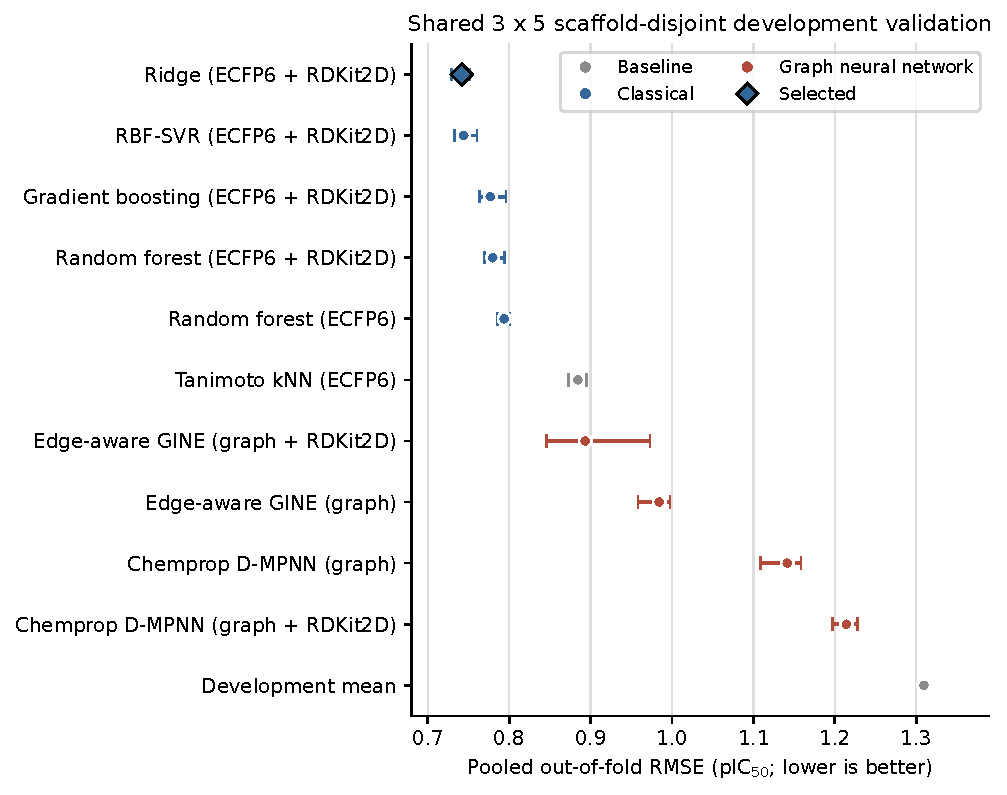
\includegraphics[width=0.94\textwidth]{figure2_development_models.pdf}
\caption{Development-only repeated scaffold-CV performance. Points show the
mean pooled out-of-fold RMSE across three repeats; bars span the minimum and
maximum repeat RMSE. Lower is better. Colors distinguish baselines, classical
fixed representations, and graph neural networks. Model selection used only the
mean repeat-level RMSE shown here.}
\label{fig:model-comparison}
\end{figure}

The \SelectedModelText{} ranked first with RMSE \DevelopmentRMSE{} and was
therefore locked before the temporal table was read. This development comparison
used deliberately modest, prespecified search spaces: the graph arm comprised
one edge-aware GINE and one Chemprop D-MPNN, each with and without descriptors,
and did not evaluate pretraining or a broad architecture search. The strongest
evaluated graph candidate was \BestGraphModelText{} (RMSE \BestGraphRMSE{}). Its paired
candidate-minus-selected RMSE difference was \BestGraphDelta{} pIC$_{50}$
(95\% scaffold-cluster bootstrap CI \BestGraphDeltaLower{} to
\BestGraphDeltaUpper{}). The runner-up \RunnerUpModelText{} was nearly tied
(RMSE \RunnerUpRMSE{}); its paired RMSE difference was \RunnerUpDelta{}
(95\% CI \RunnerUpDeltaLower{} to \RunnerUpDeltaUpper{}). Thus, selection of
Ridge follows the locked point-estimate rule and is not evidence that it is
meaningfully superior to the runner-up. Descriptor concatenation
\DescriptorAblationConclusion{}.

A post hoc audit of all \GNNCheckpointCount{} graph checkpoint manifests found
that the \GNNInnerEpochCount{} inner selected epochs ranged from
\GNNInnerEpochMinimum{} to \GNNInnerEpochMaximum{} epochs, while the
\GNNRefitEpochCount{} outer refits used \GNNRefitEpochMinimum{}--
\GNNRefitEpochMaximum{} epochs. No selected or refit epoch count equaled the
\GNNEpochCap{}-epoch ceiling, so no outer refit was assigned the cap. The
architecture and hyperparameter search nevertheless remained deliberately
narrow. Each outer graph refit used one prespecified initialization; repeated
partitions do not separately estimate optimization-seed variability, and the
paired bootstrap intervals condition on these realized fits.

Under this fixed budget, the four evaluated graph variants did not improve on
the leading ECFP6-plus-descriptor models or justify their added flexibility.
This narrow, target-specific result does not establish a general advantage of
fixed over learned representations.

\subsection{Expanded nested tuning gives graph models an architecture-tuned comparison}

We addressed the narrow graph budget in a separate post hoc analysis confined
to the \DevelopmentCount{}-compound development set (Table~\ref{tab:tuned-gnn}). In every one of
the 15 immutable outer folds, each of three graph families received
\TunedGNNCandidateBudget{} candidates: one documented baseline plus
\TunedGNNRandomDrawCount{} deterministic random draws. The search varied
learning rate, AdamW weight decay, message-passing depth and width, head width
and depth, dropout, batch size, pooling, normalization, graph featurization, and
graph-only versus descriptor-augmented input. GINE additionally varied residual
updates and Xavier versus Kaiming initialization. The Chemprop arm compared
three supported atom feature schemas, while the pretrained arm used a frozen
2,048-dimensional CheMeleon D-MPNN encoder and tuned its downstream head.

The top \TunedGNNRerankCount{} configurations from the initial single-seed screen
in each family/fold were reranked over three initialization seeds on the inner
scaffold folds. The selected configuration was then refit with
\TunedGNNSeedCount{} seeds on the complete
outer-training partition and its outer predictions were averaged. This produced
\TunedGNNInnerFitCount{} inner fits rather than treating early stopping as a
substitute for model selection. The strongest family was the
\TunedGNNBestModelText{} (RMSE \TunedGNNBestRMSE{} $\pm$
\TunedGNNBestRMSESD{} across repeats). Its paired RMSE difference versus the
original Ridge reference was \TunedGNNBestDelta{} pIC$_{50}$ (95\%
scaffold-cluster bootstrap CI \TunedGNNBestDeltaLower{} to
\TunedGNNBestDeltaUpper{}). This family-specific interval is descriptive and
was not adjusted for selecting the lowest-RMSE family among the three. For that
comparison, the point estimate slightly favored Ridge and the interval included
zero, so the expanded search did not establish a graph-model improvement over
the locked fixed-representation reference. For that
family, the mean per-compound SD across the three outer-refit predictions was
\TunedGNNBestMeanPredictionSeedSD{}
pIC$_{50}$, and the mean within-repeat SD of single-seed RMSE was
\TunedGNNBestWithinRepeatSeedRMSESD{}. Because this search was designed after
the temporal outcomes had already been inspected, it is a development-only
sensitivity: it cannot retroactively replace the prespecified selection or
supply a second confirmatory temporal comparison.

\begin{table}[H]
\centering
\caption{Post hoc development-only nested graph-model search.}
\label{tab:tuned-gnn}
\scriptsize
\setlength{\tabcolsep}{2.5pt}
\begin{tabular}{L{0.24\textwidth}L{0.10\textwidth}R{0.13\textwidth}R{0.13\textwidth}R{0.13\textwidth}R{0.20\textwidth}}
\toprule
\textbf{Family} & \textbf{Encoder} & \textbf{RMSE} & \textbf{MAE} & \textbf{$R^2$} & \textbf{$\Delta$RMSE vs Ridge [95\% CI]} \\ 
\midrule
Frozen CheMeleon + tuned head & pretrained & 0.754 $\pm$ 0.011 & 0.583 $\pm$ 0.006 & 0.668 $\pm$ 0.009 & 0.002 [-0.038, 0.046] \\
Tuned edge-aware GINE & random & 0.760 $\pm$ 0.012 & 0.596 $\pm$ 0.002 & 0.663 $\pm$ 0.010 & 0.013 [-0.027, 0.054] \\
Tuned Chemprop D-MPNN & random & 0.779 $\pm$ 0.011 & 0.613 $\pm$ 0.008 & 0.645 $\pm$ 0.010 & 0.033 [-0.016, 0.083] \\
\bottomrule
\end{tabular}
\par\vspace{3pt}\parbox{0.97\textwidth}{\footnotesize \textit{Note.} Values are mean $\pm$ population SD across three complete outer-CV repeats. Within every outer fold, each family received one anchored baseline plus 23 deterministic random draws over architecture, optimization, representation, and regularization; the top 3 were reranked over 3 initialization seeds. Outer predictions average 3 refits. Confidence intervals are paired 10,000-replicate scaffold-cluster bootstraps after averaging predictions across repeats; they are family-specific and not multiplicity-adjusted for choosing the lowest-RMSE family. This analysis was designed after the temporal results had been inspected and was not eligible to alter the locked temporal analysis.}
\end{table}


\subsection{Pooled temporal performance masked cohort-level degradation}

After development-only selection, the selected procedure was tuned on three
scaffold-disjoint folds within the complete development set, refit without
temporal labels, and evaluated once. It achieved RMSE \TemporalRMSE{} (95\% CI
\TemporalRMSELower{}--\TemporalRMSEUpper{}), MAE \TemporalMAE{} (95\% CI
\TemporalMAELower{}--\TemporalMAEUpper{}), and $R^2=\TemporalRtwo{}$ (95\% CI
\TemporalRtwoLower{}--\TemporalRtwoUpper{}; Table~\ref{tab:temporal}). Relative
to the repeated-CV RMSE, the temporal error changed by
\TemporalGeneralizationGap{} pIC$_{50}$ units. Confidence intervals resampled
Bemis--Murcko scaffold clusters, not individual compounds.

The post hoc provenance audit showed an additional boundary: development labels
came from \DevelopmentAssayCount{} assays in \DevelopmentDocumentCount{}
documents, whereas temporal labels came from \TemporalAssayCount{} assays in
\TemporalDocumentCount{} documents. The two partitions shared
\AssayPartitionOverlapCount{} assay identifiers and
\DocumentPartitionOverlapCount{} document identifiers. Temporal performance
therefore reflects joint chemical, calendar-cohort, and assay/source-provenance
shift; these components cannot be causally separated by this split.

\begin{table}[H]
\centering
\caption{One-time temporal performance and prespecified diagnostics.}
\label{tab:temporal}
\small
\begin{tabular}{L{0.40\textwidth}rrrrr}
\toprule
\textbf{Subset} & \textbf{$n$} & \textbf{Scaffolds} & \textbf{RMSE} & \textbf{MAE} & \textbf{$R^2$} \\
\midrule
Primary temporal test & 284 & 160 & 0.972 & 0.750 & 0.470 \\
New scaffold & 251 & 149 & 0.980 & 0.748 & 0.439 \\
Seen scaffold & 33 & 11 & 0.914 & 0.764 & 0.360 \\
Inside training-defined AD & 130 & 67 & 0.954 & 0.744 & 0.500 \\
Outside training-defined AD & 154 & 98 & 0.988 & 0.755 & 0.135 \\
Sensitivity: observed pIC$_{50}\leq 10$ & 277 & 159 & 0.968 & 0.741 & 0.401 \\
\bottomrule
\end{tabular}
\par\vspace{3pt}\parbox{0.94\textwidth}{\footnotesize \textit{Note.} Primary 95\% scaffold-cluster bootstrap CIs: RMSE 0.872--1.075; MAE 0.666--0.840; $R^2$ 0.311--0.582. Subgroup rows are descriptive and are not model-selection criteria. Subgroup $R^2$ values use subgroup-specific outcome variance and should not be interpreted as error-stratification evidence.}
\end{table}


\enlargethispage{2\baselineskip}
The pooled $R^2$ does not by itself describe prioritization within successive
chemistry cohorts. In a post hoc audit, annual RMSE rose from
\TemporalRMSETwentyNineteen{} in 2019 to
\TemporalRMSETwentyTwentyFour{} in 2024:
\mbox{$+\TemporalRMSEIncrease{}$ pIC$_{50}$ (\TemporalRMSEIncreasePercent{}\%)}
(95\% scaffold-cluster CI \TemporalRMSEIncreaseScaffoldLower{}--
\TemporalRMSEIncreaseScaffoldUpper{}). The four
2025 compounds were too few for an independent cohort interpretation. Annual
$R^2$ was weak or negative in most cohorts after 2019
(Table~\ref{tab:temporal-year}), and annual rank correlations were unstable
(Fig.~\ref{fig:temporal-evaluation}).

\begin{table}[H]
\centering
\caption{Post hoc descriptive temporal performance by first eligible record year. These analyses were not prespecified and were not used for model selection.}
\label{tab:temporal-year}
\scriptsize
\setlength{\tabcolsep}{2.4pt}
\begin{tabular*}{0.99\textwidth}{@{\extracolsep{\fill}}rrrrrrrrr@{}}
\toprule
\textbf{Year} & \textbf{$n$} & \textbf{Observed mean (SD)} & \textbf{Predicted mean} & \textbf{RMSE} & \textbf{MAE} & \textbf{$R^2$} & \textbf{$r$} & \textbf{$\rho_s$} \\
\midrule
2019 & 87 & 8.177 (1.334) & 8.084 & 0.795 & 0.606 & 0.645 & 0.813 & 0.842 \\
2020 & 59 & 7.329 (0.808) & 7.622 & 0.830 & 0.666 & -0.053 & 0.332 & 0.338 \\
2021 & 34 & 6.615 (0.932) & 7.015 & 0.900 & 0.647 & 0.068 & 0.506 & 0.527 \\
2022 & 25 & 6.386 (0.737) & 6.725 & 1.015 & 0.753 & -0.893 & -0.400 & -0.298 \\
2023 & 15 & 6.109 (0.939) & 6.112 & 1.234 & 0.994 & -0.727 & -0.059 & 0.032 \\
2024 & 60 & 6.511 (1.258) & 6.617 & 1.261 & 1.061 & -0.006 & 0.364 & 0.349 \\
2025$^\ast$ & 4 & 6.347 (0.408) & 6.072 & 0.590 & 0.394 & -1.089 & 0.130 & -0.200 \\
\bottomrule
\end{tabular*}
\par\vspace{2pt}\parbox{0.97\textwidth}{\footnotesize \textit{Note.} Observed SD uses the population convention. Pearson $r$ and Spearman $\rho_s$ summarize within-cohort association and are unstable in small cohorts. $^\ast$The 2025 row contains only four compounds and should not be interpreted independently.}
\end{table}


Annual cohort means accounted for \BetweenYearVariancePercent{}\% of the observed
temporal potency variance. After observed and predicted values were each centered
within first-record year, pooled $R^2$ was \WithinYearCenteredRtwoAll{} across
2019--2025. Excluding 2019, the within-year-centered $R^2$ was
\LaterCohortCenteredRtwo{} and Spearman $\rho$ was
\LaterCohortCenteredSpearman{}. Thus, the aggregate $R^2=\TemporalRtwo{}$ partly
reflects separation among annual cohorts with different mean potency, while
rank ordering within more recent cohorts was weak and unstable. This is a
cohort-composition effect, not evidence that the pooled metric is numerically
incorrect, and the year-aware analysis is descriptive rather than a second
confirmatory evaluation.

The dependence unit also mattered. Resampling document-source sets rather than
160 scaffolds gave wider sensitivity intervals: RMSE
\DocumentClusterRMSELower{}--\DocumentClusterRMSEUpper{} and $R^2$
\DocumentClusterRtwoLower{}--\DocumentClusterRtwoUpper{} (Supplementary
Table~\ref{tab:temporal-robustness}). The endpoint 2019-to-2024 RMSE contrast
included zero under document-source resampling, but a less endpoint-sensitive
linear summary of absolute error increased by \AbsoluteErrorSlopePerYear{}
pIC$_{50}$ per year (95\% scaffold-cluster CI
\AbsoluteErrorSlopeScaffoldLower{}--\AbsoluteErrorSlopeScaffoldUpper{}); its
assay- and document-source intervals also remained above zero. After centering
observed and predicted potency within source groups containing at least three
compounds, document-centered $R^2$ was \DocumentCenteredRtwo{} with
$\rho=\DocumentCenteredSpearman{}$ (\DocumentCenteredCount{} compounds in
\DocumentCenteredGroupCount{} documents), and assay-centered $R^2$ was
\AssayCenteredRtwo{} with $\rho=\AssayCenteredSpearman{}$
(\AssayCenteredCount{} compounds in \AssayCenteredGroupCount{} assays). Thus,
weak within-source ordering was not solely an artifact of annual centering.

\begin{figure}[t]
\centering
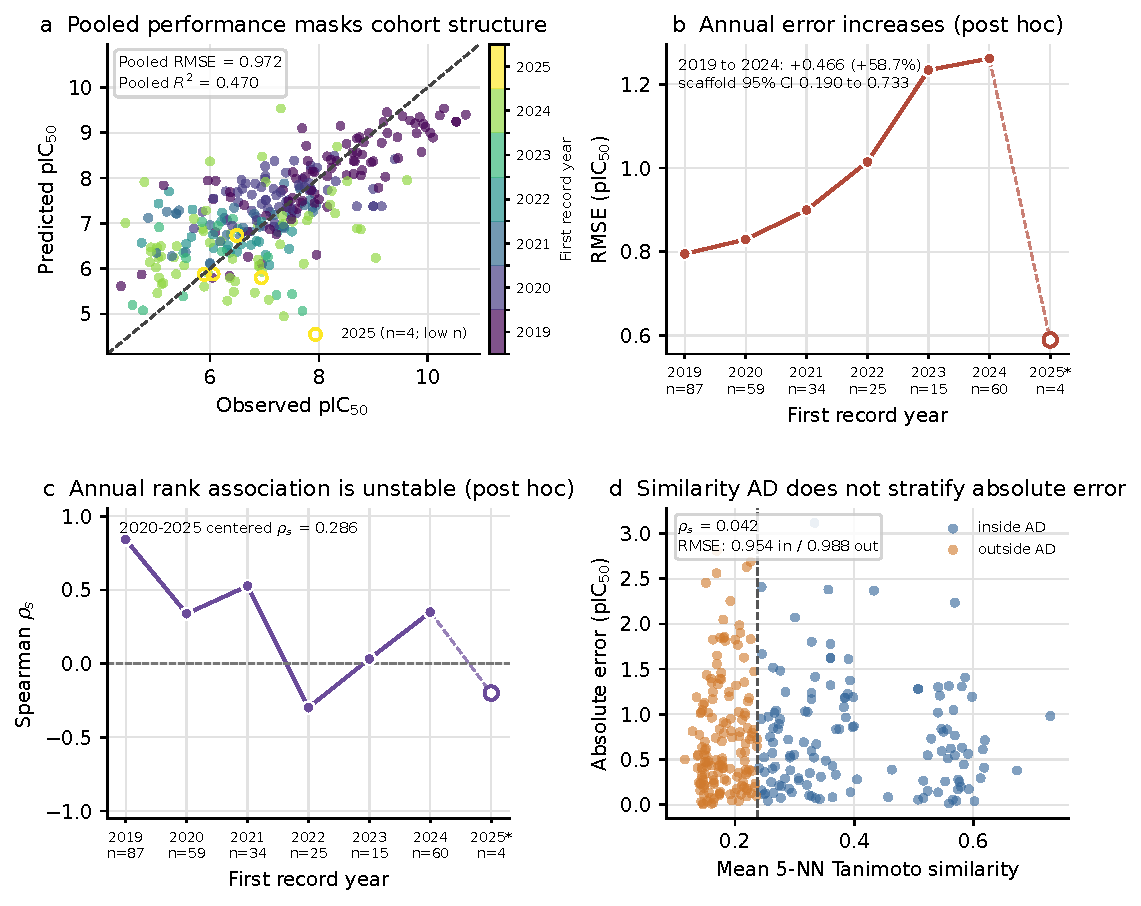
\includegraphics[width=\textwidth]{figure3_temporal_evaluation.pdf}
\caption{One-time temporal evaluation of the development-selected model.
\textbf{a}, observed versus predicted pIC$_{50}$, with the identity line.
\textbf{b}, RMSE by first eligible record year.
\textbf{c}, Spearman rank correlation by first eligible record year.
\textbf{d}, absolute error against mean Tanimoto similarity to the five nearest
development compounds, with the training-defined applicability-domain threshold.
Annual panels are post hoc descriptive audits; the 2025 estimates contain only
four compounds.}
\label{fig:temporal-evaluation}
\end{figure}

\subsection{The evaluated reliability diagnostics did not identify temporal errors}

The observed-on-predicted calibration slope was \CalibrationSlope{} with
intercept \CalibrationIntercept{}. An absolute-residual reference band defined
by the finite-sample 90\% quantile of locked development OOF errors had width
\IntervalWidth{} pIC$_{50}$ and covered \TemporalCoveragePercent{}\% of temporal
compounds (95\% scaffold-cluster CI
\CoverageLowerPercent{}--\CoverageUpperPercent{}\%). This was not a conformal
predictor: its scores came from fold-specific OOF fits after development-based
candidate selection, whereas its centers came from a separate final refit.
Moreover, ordinary exchangeability between development and future cases is not
justified under the observed temporal chemical and assay/process shift
\citep{tibshirani2019covariate,barber2023beyond}. The reported coverage is
therefore empirical, not a distribution-free guarantee. Even apart from formal
validity, the approximately \IntervalFoldSpan{}-fold IC$_{50}$ span has limited
value for typical potency-threshold decisions. Conformal regression remains a
useful QSAR framework when its construction and assumptions match the intended
deployment setting \citep{svensson2018conformal}.

The applicability-domain threshold was the fifth percentile of development
compounds' mean Tanimoto similarity to their five nearest non-self development
neighbors. \OutsideADCount{} temporal compounds fell below it. Absolute error
and mean neighbor similarity had Spearman $\rho=\SimilarityErrorRho{}$.
Inside- and outside-domain RMSE and MAE were nearly indistinguishable
(RMSE \InsideADRMSE{} versus \OutsideADRMSE{}; Table~\ref{tab:temporal}), so the threshold described structural distance but
failed to identify the predictions with larger errors. Although subgroup $R^2$
differed, outcome spread and cohort composition also differed; that
denominator-sensitive contrast should not be interpreted as evidence that the
domain discriminated reliability.
Performance on the \NewTemporalCompoundCount{} compounds with new scaffolds was
RMSE \NewScaffoldRMSE{}, compared with \SeenScaffoldRMSE{} on the
\SeenTemporalCompoundCount{} seen-scaffold compounds. These subgroup estimates
are descriptive and differ greatly in sample size.

An outcome-aware explanatory audit clarified why structural proximity alone was
insufficient. The absolute potency difference between each temporal compound and
its most similar development neighbor correlated with model absolute error
($\rho=\NearestNeighborGapErrorRho{}$; 95\% scaffold-cluster bootstrap CI
\NearestNeighborGapErrorLower{}--\NearestNeighborGapErrorUpper{}). This
nearest-neighbor potency gap uses the temporal outcome and is therefore not an
available prediction-time uncertainty score. It instead identifies response-space
discordance---the continuous analogue of an activity-cliff problem---as one
contributor to failure of the purely structural domain
\citep{vantilborg2022cliffs}.

Fifteen strict measurement events exceeded the prespecified pIC$_{50}>10$ tail
threshold. Removing the \TemporalHighTailRemoved{} such temporal compounds
yielded RMSE \NoHighTailTemporalRMSE{}. This sensitivity analysis was
prespecified because extreme public-database potency values can be influential;
it was not used to alter the primary model or endpoint.

\section{Discussion}

This study changes the evidential basis of the PIM1 analysis by replacing a
mutable or ambiguously dated dataset with a release-pinned, lineage-preserving
cohort and by enforcing immutable time and scaffold boundaries before model
comparison. Candidate selection was completed without temporal outcomes, after
which the locked procedure used the temporal set exactly once. The code paths,
null temporal-input hashes in development manifests, start record, and completed
evaluation manifest make that operational boundary auditable; they are a software
control, not a claim that the label file was cryptographically inaccessible.

The most decision-relevant result is not the pooled temporal $R^2$, but the
deterioration within successive chemistry cohorts. Error rose materially from
2019 to 2024, and the post hoc year-aware analysis found weak and unstable
within-cohort ordering after 2019. Differences among annual mean potencies
restored variation when cohorts were pooled and therefore made the aggregate
$R^2$ more favorable than recent-cohort prioritization alone. This does not make
the pooled estimate invalid; it shows that a single pooled statistic answers a
different question from whether a model can rank compounds within the chemistry
available in a particular year. Both views are needed for discovery decisions.
The added dependence audit sharpens this conclusion: source-level clustering
widened uncertainty, while error still increased in a linear time summary and
within-document and within-assay ordering remained weak. The evidence supports
degradation under joint shift, but not a source-independent causal time effect.

The negative reliability results reinforce that distinction. The locked
Tanimoto threshold detected structural distance---more than half of temporal
compounds lay outside it---but did not identify high-error predictions. Likewise,
the development-residual reference band was wide, undercovered after temporal
shift, and had limited threshold-decision value. Similarity and cross-validated
residuals therefore described aspects of the shift without yielding a useful
prediction-level reliability screen. This failure is informative: standard diagnostics that
look sensible in development may not remain operational under combined chemical,
assay, and cohort shift.
The positive association between nearest-neighbor potency discordance and model
error further indicates that response discontinuities and assay-dependent labels,
not distance alone, contribute to the failures.

More elaborate structural-domain methods can sometimes separate uncertainty
reliability on nonrandom test sets \citep{hosni2026explicit}. The negative result
here therefore concerns this simple mean-5-neighbor threshold, not the entire
applicability-domain concept; it motivates direct validation of each proposed
reliability rule under the deployment shift it is meant to address.

The representation comparison is secondary. Under the prespecified modest
search budget, none of the four evaluated graph variants improved on the leading
ECFP6-plus-descriptor candidates. The expanded development-only analysis then
tested whether that finding was merely an artifact of a single graph
architecture. It supplied equal nested candidate-count budgets, repeated initializations,
multiple pooling and normalization rules, three Chemprop feature schemas, and a
frozen pretrained D-MPNN representation. Its best result and paired uncertainty
are reported explicitly rather than inferred from the original ablation. The
best graph-family point estimate remained slightly worse than Ridge and its
paired interval included zero. Thus, the stronger experiment supports
comparability, not a claim that learned graphs outperform the fixed reference.
This
stronger comparison still does not vary training-set size, so it cannot identify
data scarcity as a cause, and it does not establish a universal ordering of
fixed and learned representations. Pretraining benefits are setting-dependent
and downstream optimization can erase apparent gains on small tasks
\citep{sun2022pretraining}; the frozen CheMeleon result should therefore be read
as one relevant transferred representation, not as an exhaustive
foundation-model leaderboard.

Publication-year validation is more decision-relevant than a random split and
more realistic than scaffold CV alone, but it remains retrospective. Because
public ChEMBL publication dates can pool distinct groups and projects, this split
enforces a chronological information boundary without reproducing the
feedback-driven order in which compounds are designed and tested within one
medicinal-chemistry program \citep{sheridan2013timesplit,landrum2023simpd}. It
therefore combines chemical novelty with changes in assay, reporting, and
deposition practice rather than isolating prospective model decay. The high
prevalence of new scaffolds and complete assay/document turnover make those
joint shifts explicit.

Several limitations bound interpretation. ChEMBL harmonizes reported endpoints
but does not make assays experimentally identical. Even confidence-9 biochemical
IC$_{50}$ values can differ in substrate, ATP concentration, construct, protocol,
and laboratory \citep{landrum2024noise,nelen2025matched}. Numeric ATP concentration was recoverable for only
\NumericATPEventPercent{}\% of strict events, only \CrossAssayCompoundCount{}
compounds bridged assays, and \AssayExclusiveScaffoldEventPercent{}\% of events
belonged to scaffolds seen in a single assay. ATP normalization would additionally
require the relevant kinetic parameters and inhibition mechanism; assay-effect
estimation is confounded by chemistry and time. We therefore did not attempt a
post hoc Cheng--Prusoff correction, assay random effect, or causal decomposition.

Document year is a publication-linked proxy for availability, not the date a
result entered ChEMBL or became accessible to a model developer. The test is
chronologically held out but arises from the same public database and
literature-curation ecosystem; it is not independent external-laboratory or
prospective validation. Median aggregation reduces replicate influence but can
hide multimodality, so event-level lineage remains essential. The expanded GNN
search corrects the original arm's narrow budget and single-initialization
assessment, but it was designed after the temporal results were known and is
therefore development-only. It covers neither every graph architecture nor every
pretraining strategy, and no newly untouched cohort was available for a fair
second temporal comparison.
Applicability-domain and calibration analyses diagnose this dataset; they do not
prove uncertainty validity after distribution shift. Finally, the endpoint is
PIM1 biochemical potency only. No inference is warranted about PIM2/PIM3
selectivity, kinome off-targets, cell permeability, toxicity, pharmacokinetics,
or efficacy.

The decisive next study is a prospectively registered evaluation in which
predictions are frozen before new outcomes are generated. It should include
deliberately selected new scaffolds, a single biochemical assay system with
reported ATP conditions, matched measurements against PIM1, PIM2, and PIM3, and
a cellular substrate-phosphorylation or target-engagement assay. Kinome
selectivity and ADME should remain separately defined endpoints. Such a study
would test whether the present error and reliability estimates translate to
genuine discovery use.

\section{Methods}

\subsection{Release snapshot and source provenance}

Data were queried from the ChEMBL REST interface for target CHEMBL2147 by
requiring the standardized IC$_{50}$ endpoint, exact equality, nM units,
standard flag~1, and a nonmissing positive value. The snapshot records ChEMBL~37,
release date 1~May~2026, the REST
base URL, the official release-status response, and the official FTP release
README, notes, and checksums. Activities, referenced assay records, target
metadata, and parent-molecule records were written as compressed JSON lines or
JSON with per-file SHA-256 values. A curation manifest links every downstream
table to those hashes. ChEMBL is described by \citet{zdrazil2024chembl}.

\subsection{Structure and activity curation}

Parent structures were processed with
\texttt{chembl-structure-pipeline==1.2.4}, which implements ChEMBL-like structure
standardization on RDKit \citep{bento2020pipeline}. The standardized parent was
serialized as canonical isomeric SMILES and identified by InChIKey. Bemis--Murcko
scaffolds were generated with RDKit \citep{bemis1996properties}; acyclic compounds
were assigned a common explicit acyclic group. The structure pipeline version was
checked at runtime and no fallback standardizer was permitted.

Broad eligibility required human PIM1 target metadata, exact positive IC$_{50}$
in nM, standard flag~1, no potential-duplicate flag, no data-validity warning, a
valid document year, concordant assay target, and a standardizable parent
structure. The strict primary cohort additionally required assay type
\texttt{B}, BAO format \texttt{BAO\_0000357} (single protein), target relationship
\texttt{D}, confidence score~9, and no variant accession or mutation. Equivalent
source events were identified from parent, target, record, document, normalized
assay description, endpoint, format, assay type, relation, value, and units; their
activity identifiers remained in a lineage table.

Activity was transformed as
\[
  \mathrm{pIC}_{50}=9-\log_{10}(\mathrm{IC}_{50}\;[\mathrm{nM}]).
\]
Compound labels were the median eligible event pIC$_{50}$. Counts, standard
deviation, median absolute deviation, range, first and last document year, event
IDs, assay IDs, and document IDs were retained. The prespecified high-tail
sensitivity cohort excluded events with pIC$_{50}>10$.

\subsection{Post hoc assay-metadata audit}

After the sealed evaluation, we audited assay context directly from the pinned
strict event table; this audit was descriptive and did not alter labels, model
selection, or predictions. Events were grouped by representative assay,
document, standardized-parent identity, and Bemis--Murcko scaffold. We counted
case-insensitive whole-word mentions of ATP. Explicit positive concentrations
were extracted only when a numeric nM, $\mu$M, or mM value immediately modified
ATP in the archived description; values were normalized to $\mu$M. Descriptions
stating ATP at $K_m$ without a numeric value were tabulated separately. Missing
text was never interpreted as a constant or absent ATP condition.

Assay-size distributions, cross-assay compound bridges, and the proportion of
events whose scaffold occurred in only one assay were computed without reference
to prediction error. Development provenance used label events at or before the
2018 cutoff; quarantined later records for development identities were excluded.
All events for first-seen-after-cutoff identities defined temporal provenance.
Assay and document intersections were then enumerated across partitions. Finally,
we exhaustively searched for identities measured within the same document in
different assays with different explicit ATP concentrations; no pair was selected
by the direction or magnitude of its potency change. Because assay conditions,
chemistry, and time were sparsely bridged, this audit was not used to fit an
assay-effect model or normalize IC$_{50}$.

\subsection{Outcome-blind temporal sealing}

Compound identity was assigned to development or temporal test by its first
eligible strict measurement-event document year. Before any candidate model was
fit, a count-only feasibility table enumerated each potential cutoff. The locked
rule chose the latest cutoff with at least 750 development compounds, 250
temporal compounds, and 100 scaffolds present only in the temporal partition.
No activity value was permitted in cutoff selection. The selected cutoff was
2018, so development used events through 2018 and the test contained compounds
first meeting the strict cohort definition from 2019 onward. Post-2018 records for identities already assigned
to development were quarantined and never updated training labels. Development,
temporal, cross-cutoff, and fold-assignment files were made immutable through a
split manifest containing source and output hashes.

This construction is a retrospective publication-year temporal split, not a
prospective experiment. It follows the rationale that time-split validation can
better approximate future prediction than random resampling
\citep{sheridan2013timesplit}, while recognizing that simulated or historical
splits have their own biases \citep{landrum2023simpd}.

\subsection{Fixed molecular representations and classical candidates}

ECFP6 fingerprints were generated with radius~3 and 2,048 bits
\citep{rogers2010extended}. A 23-variable RDKit descriptor vector contained
molecular weight, calculated logP, hydrogen-bond counts, rotatable bonds, ring and
aromatic-ring counts, heteroatom and heavy-atom counts, fraction sp$^3$, TPSA,
Labute ASA, Balaban $J$, Bertz complexity, molecular connectivity indices, QED,
formal charge, and related atom-count descriptors. The exact ordered descriptor
list is stored in the feature manifest.

Seven prespecified fixed-representation or baseline candidates were evaluated: a training-mean baseline,
unweighted Tanimoto $k$-nearest-neighbor regression on ECFP6, Ridge regression,
random forest on ECFP6, random forest on ECFP6 plus descriptors, gradient boosting
on the combined representation, and RBF support-vector regression on the combined
representation. Median imputation and, where appropriate, descriptor scaling were
inside each scikit-learn pipeline. Hyperparameter grids are reported in
Supplementary Table~\ref{tab:hyperparameters}.

\subsection{Graph neural networks}

Four graph candidates crossed two backends with two feature variants: molecular
graph alone and graph plus the same 23 RDKit descriptors. The custom edge-aware
GINE used explicit atom and bond features, three message-passing layers, hidden
dimension 128, residual updates, batch normalization, mean pooling, a two-layer
feed-forward head, and dropout 0.1. Its edge-aware convolution followed the GINE
operator used in graph representation learning \citep{hu2020strategies}; the
implementation used PyTorch Geometric \citep{fey2019pyg}.

The second backend used Chemprop~2.2.4 bond-directed message passing, mean
aggregation, hidden dimension 128, depth~3, and a matched 128-dimensional
feed-forward head \citep{yang2019analyzing,graff2026chempropv2}. Both backends used batch size~64,
Adam-family optimization, target scaling estimated from the current training
partition, maximum 80 epochs, and patience~10 with a minimum RMSE improvement of
0.001. Descriptor variants median-imputed and standardized descriptors from the
current training rows only.

\subsection{Post hoc expanded graph-model tuning}

After the prespecified temporal analysis and its robustness audit had been
completed, we designed a separate development-only graph search. It reused the
immutable 3$\times$5 outer scaffold assignments but neither loaded nor predicted
the temporal table. Three families were compared: a task-trained edge-aware
GINE, a task-trained Chemprop D-MPNN, and the CheMeleon D-MPNN encoder described
in a 2025 preprint and pretrained to predict molecular descriptors for one
million PubChem structures \citep{burns2025chemeleon}. CheMeleon was used as a
frozen 2,048-dimensional
representation so that encoder pretraining was cleanly separated from the
PIM1-labeled head fit. The upstream checkpoint was obtained from Zenodo record
15460715 \citep{burns2025chemeleonmodel} and verified against SHA-256
\nolinkurl{c376624d3407204e780a0ed13a9ac097cc9bb1c13ef89cdbc633c1715c183651}.
Because its descriptor-pretraining corpus may contain structures represented in
ChEMBL, this arm tests transferred structural representation, not a claim of
structure-level non-exposure or PIM1-label pretraining.

Within each outer-training partition, all families used the same three
scaffold-disjoint inner folds and a deterministic
\TunedGNNCandidateBudget{}-candidate budget comprising one documented baseline
and \TunedGNNRandomDrawCount{} random draws; the same family-specific candidate
set was evaluated independently in every outer fold
(Table~\ref{tab:tuned-gnn-search-space}). Random search is efficient when only a
subset of hyperparameters is consequential \citep{bergstra2012random}; per-model
tuning and repeated initializations also follow the central fairness controls
used in MoleculeNet and controlled GNN comparisons
\citep{wu2018moleculenet,errica2020fair}. The sampled space covered learning rate
($10^{-5}$--$3\times10^{-3}$), AdamW weight decay (zero or
$10^{-8}$--$10^{-3}$), depth (2--6 for task-trained encoders), message and head
width (64--512), head depth (1--3), dropout (0--0.4), batch size (32, 64, or
128), pooling, normalization, descriptor fusion, and backend-specific feature
and residual choices. Chemprop atom featurization varied among its v1, v2, and
organic schemas. GINE varied mean versus additive pooling, no/batch/layer
normalization, residual updates, and Xavier versus Kaiming uniform
initialization. The pretrained encoder architecture and v2 atom features were
fixed by its checkpoint; its downstream head and descriptor fusion were tuned.

Each configuration was first scored by pooled inner out-of-fold RMSE. The top
three configurations per family and outer fold were then refit across seeds
7301, 7302, and 7303 and ranked by mean pooled inner RMSE, with candidate hash as
an exact-tie breaker. For the selected configuration, the median inner-selected
epoch for each seed was assigned to a fresh full outer-training refit. Outer
predictions from seeds 8101, 8102, and 8103 were averaged, while seed-specific
predictions were retained. Target and descriptor scalers were fitted only on
the current inner-training rows and then applied to validation rows. AdamW
weight decay was implemented explicitly for both task-trained backends. GINE
early stopping monitored raw-unit RMSE; Chemprop monitored validation RMSE under
the training-fold target scaler, with its minimum improvement and reported score
exactly converted to pIC$_{50}$. These changes correct the optimizer and
validation-metric asymmetries in the original bounded graph runner. Primary
family summaries again pooled all \DevelopmentCount{} outer predictions within each repeat.
Paired differences from the original Ridge OOF reference averaged each
compound's predictions across repeats and used 10,000 scaffold-cluster bootstrap
replicates.

\subsection{Nested repeated scaffold validation and model selection}

Development validation used three repeats of five-fold
\texttt{StratifiedGroupKFold}. Bemis--Murcko scaffold was the group and ranked
pIC$_{50}$ values were divided into five approximately equal strata. Seeds 1101,
1102, and 1103 created one immutable assignment table shared across all model
families. Within each outer training partition, classical grids used three
scaffold-disjoint inner folds with all preprocessing refit inside the pipeline.
This fully nested design prevents the selection bias that results when tuning and
assessment reuse the same observations \citep{varma2006bias}.

For GNNs, the same outer partitions were used. Each outer training set was divided
into three inner scaffold folds. Early stopping was performed independently on
each inner validation fold; the median of the three selected epoch counts was
then used for a fresh fit on the entire outer training partition. Outer validation
labels were never monitored. Fixed GNN architectural settings bounded the
comparison and kept every outer fold strictly assessment-only.

After completion, selected epoch counts and assigned refit durations were read
from all graph checkpoint manifests, and each companion prediction hash was
reverified. We compared every inner selected epoch and outer refit duration with
the fixed 80-epoch ceiling. This checkpoint audit did not reconstruct how many
epochs each inner loop evaluated before early stopping; it was descriptive and
did not trigger new training or candidate changes.

RMSE was the prespecified primary metric; MAE and $R^2$ were secondary. For each
repeat, metrics were computed after pooling its complete set of 803 out-of-fold
predictions. Candidates were ranked by mean repeat-level RMSE, with model name as
an exact-tie breaker. For descriptive paired comparisons, predictions were first
averaged across repeats for each compound, then scaffold clusters were resampled
10,000 times to estimate candidate-minus-selected RMSE and MAE intervals. The
sealed temporal table was not read during selection.

\subsection{Final fitting, temporal metrics, uncertainty, and domain}

The selected classical candidate underwent a final three-fold, scaffold-disjoint
grid search on all development compounds and was refit before temporal prediction.
Had a GNN been selected, the prespecified procedure would have averaged three
development-only refits with seeds 2101--2103; that conditional procedure was
implemented before the temporal evaluation. Primary temporal RMSE, MAE, and
$R^2$ were accompanied by 95\% percentile intervals from 10,000 bootstrap samples
of temporal Bemis--Murcko scaffolds (seed 3101).

After the sealed primary evaluation, we performed a post hoc descriptive audit
by first eligible record year; it was not used to select, tune, or refit the
model. Annual RMSE, $R^2$, and Spearman correlation were calculated separately.
The fraction of observed temporal variance between years was the weighted
between-cohort sum of squares divided by the total observed sum of squares. To
separate within-cohort ordering from annual mean differences, observed and
predicted pIC$_{50}$ values were each centered by their corresponding
first-record-year mean before pooled $R^2$ and Spearman correlation were
calculated. We report this centered analysis for all temporal years and, to
describe a horizon at least two years beyond the 2018 cutoff, for 2020--2025.
Small annual
cohorts, especially 2025, make individual-year estimates unstable.

A separate, hash-linked post hoc robustness audit consumed the immutable temporal
predictions without fitting, tuning, or changing any prediction. It (i) checked
strict-cohort first-record years against the broader curated event history;
(ii) repeated primary metric intervals by resampling sorted assay-source and
document-source sets as dependence sensitivities; (iii) bootstrapped the
2019-to-2024 RMSE difference and the individual-level linear slope of absolute
error on first-record year; and (iv) centered observed and predicted pIC$_{50}$
within assay or document groups with at least three compounds. Source-set labels
preserved the two multi-document and four multi-assay compound labels rather than
assigning them arbitrarily to one source. All resampling used 10,000 replicates;
these post hoc intervals characterize dependence sensitivity and do not replace
the prespecified scaffold-cluster interval.

We applied the finite-sample order-statistic correction used in absolute-residual
conformal intervals to the selected model's locked repeat-0 development OOF
residuals. The resulting symmetric band is reported only as a reproducible
development-residual reference: its scores came from fold-specific OOF models
after development-based candidate selection, while its centers came from a
separate final refit. Moreover, the exchangeability condition required by
ordinary conformal validity is not justified for the chronologically shifted
cases \citep{barber2023beyond}. Weighted conformal methods can address pure
covariate shift under additional assumptions, including a stable conditional
outcome distribution and a known or estimable train/test density ratio
\citep{tibshirani2019covariate}; those assumptions were neither established nor
used here. Temporal coverage was therefore evaluated empirically and
scaffold-cluster bootstrapped. Calibration was summarized by the slope and
intercept from observed-on-predicted linear regression and by five equal-count
prediction bins.

The applicability domain was defined entirely from training structures. For every
development compound, mean Tanimoto similarity to its five nearest non-self
development neighbors was calculated; the fifth percentile was locked as the
threshold. Each temporal compound's mean and maximum similarity to development,
nearest neighbor, and in/out-domain status were recorded. We additionally report
error--similarity correlations and metrics by in/out-domain and new/seen-scaffold
groups. Small subgroup comparisons are descriptive rather than hypothesis tests.
For explanation only, we also calculated each temporal compound's absolute
pIC$_{50}$ difference from its most similar development neighbor and
scaffold-cluster bootstrapped its Spearman association with model absolute error.

\subsection{Software, integrity checks, and reproducibility}

Classical analysis used Python~\ClassicalPythonVersion{}, RDKit~\RDKitVersion{},
NumPy~\NumPyVersion{}, pandas~\PandasVersion{}, and scikit-learn~\SklearnVersion{}.
GNN analysis used PyTorch~\TorchVersion{}, PyTorch Geometric~\PyGVersion{}, and
Chemprop~\ChempropVersion{} in an isolated CPU environment. Environment manifests
record executable paths, installed-package inventories, platform details, and
hashes. Unit and contract tests verify curation filters, standardization behavior,
split disjointness, assignment inventories, training-only transforms, resumable
checkpoints, model-selection blindness, and one-time temporal artifact sealing.
Every production stage writes atomic files and a completion marker. SHA-256-linked
manifests cover the release, curation, split, selection, temporal-evaluation,
post hoc robustness-audit, expanded graph search, and manuscript stages. The
original GNN benchmark records its fixed contract and fold/checkpoint inventory;
the expanded benchmark additionally records every inner trial, selected
configuration, initialization-specific prediction, ensemble prediction,
pretrained checkpoint hash, and paired-bootstrap result.

\section{Data and code availability}

Code and confirmatory artifacts are available in the public GitHub repository
\url{https://github.com/OWNER/biodd_pim1_qsar_v2}
% TODO: replace OWNER with the public repository owner
and an archival Zenodo snapshot (\texttt{doi:10.5281/zenodo.XXXXXXX}).
% TODO: replace XXXXXXX with the deposited Zenodo record ID
The archive contains the exact source snapshot, release metadata, curation
tables, event lineage, immutable split, candidate predictions, selection record,
temporal predictions, figures, environment manifests, and manuscript source. The
hash-linked post hoc audit additionally contains source-set assignments,
strict-versus-broad chronology flags, and all alternative cluster intervals. The
expanded graph archive contains its search contract, 4,050 inner-fit records,
selected configurations, seed-specific and ensemble OOF predictions, and the
hash-pinned pretrained encoder provenance. The
file \texttt{ARTIFACT\_INDEX.md} identifies confirmatory v2 artifacts and clearly
separates them from legacy exploratory results. ChEMBL-derived tables are
redistributed under {CC BY-SA}~3.0 with attribution to ChEMBL~37
\citep{zdrazil2024chembl}.

\section{Conclusion}

Release pinning and sealing converted this from an algorithm demonstration into
an auditable reliability test. Pooled temporal performance remained moderate,
but source-cluster sensitivity widened its uncertainty; error increased over time
and within-year, within-document, and within-assay ranking was weak amid
inseparable chemical and assay-provenance turnover. The similarity domain did not identify
high-error predictions; the residual reference band was wide and undercovered.
Under the prespecified budget, graph models did not justify added flexibility.
The expanded nested graph sensitivity produced best development RMSE
\TunedGNNBestRMSE{} under a far broader and seed-repeated search, resolving the
most important model-comparison weakness without reusing the temporal cohort for
confirmation. The decisive next test is prospective, assay-consistent chemistry.

\section*{Author contributions}
T.N.: conceptualization, methodology, software, validation, formal analysis,
investigation, data curation, visualization, writing, and project administration.

\section*{Competing interests}
The author declares no competing interests.

\section*{Funding}
This work received no external funding.

\section*{Use of computational tools}
AI/LLM-based coding and writing assistants were used for code development,
testing, and manuscript editing.
% TODO: name the specific AI/LLM tools used.
No AI tool is an author. The author designed the study, verified all code,
outputs, and claims, and takes full responsibility for the work.

\par\bigskip
\appendix
\section{Supplementary methods and results}

\subsection{Prespecified candidate settings}
\begin{longtable}{L{0.25\textwidth}L{0.19\textwidth}L{0.48\textwidth}}
\caption{Prespecified candidate representations and search spaces.}\label{tab:hyperparameters}\\
\toprule
\textbf{Candidate} & \textbf{Representation} & \textbf{Settings or inner grid} \\
\midrule
\endfirsthead
\toprule
\textbf{Candidate} & \textbf{Representation} & \textbf{Settings or inner grid} \\
\midrule
\endhead
Development mean & none & fixed \\
Tanimoto kNN (ECFP6) & ECFP6 & n\_neighbors: [3, 5, 10, 20] \\
Ridge (ECFP6 + RDKit2D) & ECFP6 + 23 descriptors & alpha: [0.1, 1.0, 10.0, 100.0] \\
Random forest (ECFP6) & ECFP6 & max\_depth: [None, 20]; max\_features: [sqrt, 0.25]; min\_samples\_leaf: [1, 3]; n\_estimators: [200] \\
Random forest (ECFP6 + RDKit2D) & ECFP6 + 23 descriptors & max\_depth: [None, 20]; max\_features: [sqrt, 0.25]; min\_samples\_leaf: [1, 3]; n\_estimators: [200] \\
Gradient boosting (ECFP6 + RDKit2D) & ECFP6 + 23 descriptors & learning\_rate: [0.03, 0.1]; max\_depth: [2]; n\_estimators: [100, 250] \\
RBF-SVR (ECFP6 + RDKit2D) & ECFP6 + 23 descriptors & C: [1.0, 10.0, 100.0]; epsilon: [0.1, 0.2]; gamma: [scale, 0.001] \\
Edge-aware GINE (graph) & molecular graph & hidden=128; depth=3; dropout=0.1; max epochs=80; patience=10 \\
Edge-aware GINE (graph + RDKit2D) & graph + 23 descriptors & hidden=128; depth=3; dropout=0.1; max epochs=80; patience=10 \\
Chemprop D-MPNN (graph) & molecular graph & hidden=128; depth=3; dropout=0.1; max epochs=80; patience=10 \\
Chemprop D-MPNN (graph + RDKit2D) & graph + 23 descriptors & hidden=128; depth=3; dropout=0.1; max epochs=80; patience=10 \\
\bottomrule
\end{longtable}


\subsection{Curation exclusions}
\begin{table}[H]
\centering
\caption{Logged record-level and sensitivity-cohort exclusions.}
\label{tab:curation-exclusions}
\small
\begin{tabular}{L{0.20\textwidth}L{0.56\textwidth}r}
\toprule
\textbf{Cohort} & \textbf{Reason} & \textbf{Count} \\
\midrule
strict & assay confidence not strict & 2,973 \\
strict & assay relationship not direct & 2,973 \\
broad & duplicate source event collapsed & 1,024 \\
broad & potential duplicate & 473 \\
strict & bao format not single protein & 402 \\
strict\_no\_high\_tail & pIC50 above prespecified threshold & 15 \\
broad & data validity warning & 11 \\
strict & assay type not biochemical & 1 \\
\bottomrule
\end{tabular}
\end{table}


\subsection{Post hoc assay-context audit}
\begin{table}[H]
\centering
\caption{Post hoc audit of strict assays whose pinned descriptions state a numeric ATP concentration or ATP at $K_m$.}
\label{tab:assay-context}
\scriptsize
\setlength{\tabcolsep}{3pt}
\begin{tabular}{L{0.23\textwidth}L{0.23\textwidth}rL{0.27\textwidth}}
\toprule
\textbf{Assay} & \textbf{Reported ATP condition} & \textbf{Events} & \textbf{Document(s)} \\
\midrule
CHEMBL1061942 & 20 $\mu$M & 4 & CHEMBL1150976 \\
CHEMBL1919015 & 30 $\mu$M & 53 & CHEMBL1914433 \\
CHEMBL2020770 & 30 $\mu$M & 40 & CHEMBL2016532 \\
CHEMBL2049739 & 50 $\mu$M & 10 & CHEMBL2046384 \\
CHEMBL2049742 & 5 mM & 7 & CHEMBL2046384 \\
CHEMBL4011954 & 1 mM & 1 & CHEMBL4011589 \\
CHEMBL4831324 & 1 mM & 1 & CHEMBL4828769 \\
CHEMBL4831325 & 1 mM & 1 & CHEMBL4828769 \\
CHEMBL4687896 & ATP = $K_m$ (value unstated) & 1 & CHEMBL4680285 \\
CHEMBL5212833 & ATP = $K_m$ (value unstated) & 1 & CHEMBL5212743 \\
CHEMBL5446217 & ATP = $K_m$ (value unstated) & 1 & CHEMBL5446079 \\
\bottomrule
\end{tabular}
\par\vspace{2pt}\parbox{0.94\textwidth}{\scriptsize \textit{Note.} This text audit is a lower bound on ATP metadata completeness: absence of a machine-readable concentration does not imply that ATP was absent or constant. An exhaustive within-document identity bridge search found one matched compound, in CHEMBL2046384, measured at 50 $\mu$M and 5 mM (9 versus 100 nM; $\Delta$pIC$_{50}=-1.046$). This $n=1$ observation is illustrative, not an assay correction or causal estimate \citep{dakin2012pim}.}
\end{table}


\subsection{Post hoc temporal robustness audit}
\begin{table}[H]
\centering
\caption{Post hoc robustness audits of the immutable temporal predictions.}
\label{tab:temporal-robustness}
\small
\begin{tabular}{L{0.28\textwidth}rrrr}
\toprule
\textbf{Resampling unit} & \textbf{Clusters} & \textbf{RMSE 95\% CI} & \textbf{$R^2$ 95\% CI} & \textbf{$\Delta$RMSE 95\% CI} \\
\midrule
Bemis--Murcko scaffold & 160 & 0.871--1.077 & 0.312--0.582 & 0.190--0.733 \\
Assay-source set & 49 & 0.835--1.144 & -0.040--0.660 & 0.155--0.753 \\
Document-source set & 38 & 0.787--1.150 & -0.007--0.682 & -0.121--0.706 \\
\bottomrule
\end{tabular}
\par\vspace{3pt}\parbox{0.94\textwidth}{\footnotesize \textit{Note.} All intervals use 10,000 percentile-bootstrap replicates. $\Delta$RMSE is 2024 minus 2019. Assay- and document-source sets are sorted combinations of the sources contributing to each aggregated compound label; they are dependence-sensitivity analyses, not replacements for the prespecified scaffold bootstrap. The strict-chronology sensitivity excluded 4 compounds with an earlier broad-cohort record and gave RMSE 0.976 and $R^2=0.463$.}
\end{table}


\subsection{Per-repeat development metrics}
\begingroup
\small
\begin{longtable}{L{0.40\textwidth}rrrrr}
\caption{Complete pooled out-of-fold metrics by repeat.}\label{tab:repeat-metrics}\\
\toprule
\textbf{Candidate} & \textbf{Repeat} & \textbf{$n$} & \textbf{RMSE} & \textbf{MAE} & \textbf{$R^2$} \\
\midrule
\endfirsthead
\toprule
\textbf{Candidate} & \textbf{Repeat} & \textbf{$n$} & \textbf{RMSE} & \textbf{MAE} & \textbf{$R^2$} \\
\midrule
\endhead
Chemprop D-MPNN (graph) & 1 & 803 & 1.159 & 0.946 & 0.216 \\
Chemprop D-MPNN (graph) & 2 & 803 & 1.158 & 0.927 & 0.217 \\
Chemprop D-MPNN (graph) & 3 & 803 & 1.109 & 0.915 & 0.283 \\
Chemprop D-MPNN (graph + RDKit2D) & 1 & 803 & 1.218 & 1.001 & 0.135 \\
Chemprop D-MPNN (graph + RDKit2D) & 2 & 803 & 1.197 & 0.979 & 0.163 \\
Chemprop D-MPNN (graph + RDKit2D) & 3 & 803 & 1.228 & 0.998 & 0.120 \\
Development mean & 1 & 803 & 1.309 & 1.079 & -0.001 \\
Development mean & 2 & 803 & 1.309 & 1.079 & -0.001 \\
Development mean & 3 & 803 & 1.309 & 1.078 & -0.001 \\
Edge-aware GINE (graph) & 1 & 803 & 0.998 & 0.786 & 0.419 \\
Edge-aware GINE (graph) & 2 & 803 & 0.997 & 0.781 & 0.419 \\
Edge-aware GINE (graph) & 3 & 803 & 0.958 & 0.731 & 0.464 \\
Edge-aware GINE (graph + RDKit2D) & 1 & 803 & 0.973 & 0.762 & 0.447 \\
Edge-aware GINE (graph + RDKit2D) & 2 & 803 & 0.846 & 0.668 & 0.582 \\
Edge-aware GINE (graph + RDKit2D) & 3 & 803 & 0.861 & 0.674 & 0.567 \\
Gradient boosting (ECFP6 + RDKit2D) & 1 & 803 & 0.770 & 0.605 & 0.653 \\
Gradient boosting (ECFP6 + RDKit2D) & 2 & 803 & 0.764 & 0.598 & 0.659 \\
Gradient boosting (ECFP6 + RDKit2D) & 3 & 803 & 0.796 & 0.624 & 0.630 \\
Random forest (ECFP6 + RDKit2D) & 1 & 803 & 0.775 & 0.605 & 0.649 \\
Random forest (ECFP6 + RDKit2D) & 2 & 803 & 0.770 & 0.605 & 0.654 \\
Random forest (ECFP6 + RDKit2D) & 3 & 803 & 0.794 & 0.617 & 0.632 \\
Random forest (ECFP6) & 1 & 803 & 0.795 & 0.619 & 0.631 \\
Random forest (ECFP6) & 2 & 803 & 0.785 & 0.603 & 0.640 \\
Random forest (ECFP6) & 3 & 803 & 0.801 & 0.616 & 0.625 \\
RBF-SVR (ECFP6 + RDKit2D) & 1 & 803 & 0.733 & 0.571 & 0.686 \\
RBF-SVR (ECFP6 + RDKit2D) & 2 & 803 & 0.738 & 0.562 & 0.682 \\
RBF-SVR (ECFP6 + RDKit2D) & 3 & 803 & 0.761 & 0.580 & 0.662 \\
Ridge (ECFP6 + RDKit2D) & 1 & 803 & 0.744 & 0.578 & 0.677 \\
Ridge (ECFP6 + RDKit2D) & 2 & 803 & 0.730 & 0.562 & 0.689 \\
Ridge (ECFP6 + RDKit2D) & 3 & 803 & 0.752 & 0.582 & 0.670 \\
Tanimoto kNN (ECFP6) & 1 & 803 & 0.873 & 0.660 & 0.555 \\
Tanimoto kNN (ECFP6) & 2 & 803 & 0.895 & 0.676 & 0.532 \\
Tanimoto kNN (ECFP6) & 3 & 803 & 0.885 & 0.667 & 0.543 \\
\bottomrule
\end{longtable}
\endgroup


\subsection{Post hoc graph-search selections}
\begin{table}[H]
\centering
\caption{Hyperparameters selected independently in the 15 outer folds of each post hoc graph family.}
\label{tab:tuned-gnn-selections}
\scriptsize
\setlength{\tabcolsep}{3pt}
\begin{tabular}{L{0.25\textwidth}L{0.22\textwidth}L{0.22\textwidth}L{0.22\textwidth}}
\toprule
\textbf{Selection summary} & \textbf{GINE} & \textbf{D-MPNN} & \textbf{CheMeleon} \\ 
\midrule
Descriptor fusion (yes/no) & yes: 15 & no: 13; yes: 2 & no: 11; yes: 4 \\
Depth, median [range] & 3 [3, 3] & 5 [2, 5] & 6 [6, 6] \\
Message width, median [range] & 128 [128, 256] & 512 [256, 512] & 2048 [2048, 2048] \\
Head width, median [range] & 128 [128, 512] & 256 [256, 256] & 256 [256, 512] \\
Head layers, median [range] & 2 [2, 3] & 3 [2, 3] & 3 [3, 3] \\
Dropout, median [range] & 0.100 [0.100, 0.121] & 0.010 [0.010, 0.294] & 0.082 [0.082, 0.387] \\
Learning rate, median [range] & 0.000300 [0.000171, 0.000300] & 0.000248 [0.000248, 0.000312] & 0.001507 [0.000301, 0.001507] \\
Nonzero weight decay & 15/15 & 15/15 & 15/15 \\
Batch-size selections & 32: 1; 64: 14 & 128: 13; 32: 2 & 128: 15 \\
Pooling selections & mean: 15 & norm: 13; sum: 2 & mean: 15 \\
Normalization selections & batch: 14; none: 1 & batch: 15 & none: 15 \\
Residual updates (yes/no) & yes: 15 & no: 15 & no: 15 \\
Initialization selections & kaiming uniform: 1; xavier uniform: 14 & chemprop default: 15 & pretrained chemeleon: 15 \\
Activation selections & relu: 15 & relu: 15 & leakyrelu: 11; relu: 4 \\
Featurization selections & rich atom bond v1: 15 & chemprop v1: 13; chemprop v2: 2 & chemprop v2: 15 \\
\bottomrule
\end{tabular}
\par\vspace{3pt}\parbox{0.95\textwidth}{\footnotesize \textit{Note.} Counts are out of 15 outer folds. Numeric entries are median [minimum, maximum]. CheMeleon depth, message width, mean pooling, and v2 featurization were fixed by the pretrained encoder contract; its downstream head and descriptor fusion were tuned. Its initialization entry denotes the frozen pretrained encoder; each downstream head used seeded Xavier initialization.}
\end{table}


\subsection{Exact post hoc graph-search space}
\begingroup\scriptsize
\begin{longtable}{L{0.18\textwidth}L{0.225\textwidth}L{0.225\textwidth}L{0.225\textwidth}}
\caption{Exact post hoc graph-model candidate spaces and anchored baselines.}\label{tab:tuned-gnn-search-space}\\
\toprule
\textbf{Choice} & \textbf{GINE} & \textbf{D-MPNN} & \textbf{Frozen CheMeleon} \\ 
\midrule
\endfirsthead
\multicolumn{4}{l}{\footnotesize\textit{Table \thetable\ continued}}\\
\toprule
\textbf{Choice} & \textbf{GINE} & \textbf{D-MPNN} & \textbf{Frozen CheMeleon} \\ 
\midrule
\endhead
\midrule\multicolumn{4}{r}{\footnotesize\textit{Continued on next page}}\\
\endfoot
\bottomrule
\endlastfoot
Candidate construction & 1 baseline + 23 draws; seed 62017 & 1 baseline + 23 draws; seed 63026 & 1 baseline + 23 draws; seed 64035 \\
Representation & graph, graph + RDKit2D & graph, graph + RDKit2D & graph, graph + RDKit2D \\
Encoder depth & 2, 3, 4, 5, 6 & 2, 3, 4, 5, 6 & 6 (fixed) \\
Message width & 64, 128, 256, 512 & 64, 128, 256, 512 & 2,048 (fixed) \\
Head width & 64, 128, 256, 512 & 64, 128, 256, 512 & 64, 128, 256, 512 \\
Head layers & 1, 2, 3 & 1, 2, 3 & 1, 2, 3 \\
Dropout & continuous uniform [0, 0.4] & continuous uniform [0, 0.4] & continuous uniform [0, 0.4] \\
Learning rate & log-uniform [$10^{-5}$, $3\times10^{-3}$] & log-uniform [$10^{-5}$, $3\times10^{-3}$] & log-uniform [$10^{-5}$, $3\times10^{-3}$] \\
AdamW weight decay & 0, $10^{-8}$, $10^{-7}$, $10^{-6}$, $10^{-5}$, $10^{-4}$, $10^{-3}$ & 0, $10^{-8}$, $10^{-7}$, $10^{-6}$, $10^{-5}$, $10^{-4}$, $10^{-3}$ & 0, $10^{-8}$, $10^{-7}$, $10^{-6}$, $10^{-5}$, $10^{-4}$, $10^{-3}$ \\
Batch size & 32, 64, 128 & 32, 64, 128 & 32, 64, 128 \\
Pooling & mean, sum & mean, sum, size-normalized sum & mean (fixed) \\
Normalization & none, batch, layer & none, batch & none, batch \\
Residual updates & no, yes & no (fixed) & no (fixed) \\
Initialization & Xavier uniform, Kaiming uniform & Chemprop default (seeded) & pretrained encoder; Xavier head \\
Activation & ReLU (fixed) & ReLU, leaky ReLU, ELU & ReLU, leaky ReLU, ELU \\
Atom/bond features & rich atom/bond v1 & Chemprop v1, Chemprop v2, Chemprop organic & Chemprop v2 (fixed) \\
Encoder training & task-trained & task-trained & frozen \\
Baseline: representation / encoder / head & graph + RDKit2D; 3 $\times$ 128; 2 $\times$ 128 & graph; 3 $\times$ 128; 2 $\times$ 128 & graph; 6 $\times$ 2,048 frozen; 2 $\times$ 128 \\
Baseline: dropout / learning rate / weight decay / batch & 0.1 / $3\times10^{-4}$ / $10^{-5}$ / 64 & 0.1 / $3\times10^{-4}$ / 0 / 64 & 0.1 / $3\times10^{-4}$ / $10^{-5}$ / 64 \\
Baseline: pool / normalization / activation & mean / batch / ReLU & mean / batch / ReLU & mean / batch / ReLU \\
\multicolumn{4}{L{0.84\textwidth}}{\footnotesize \textit{Note.} Each family received one anchored baseline plus 23 deterministic random draws; the same family-specific candidate set was evaluated in every outer fold. Dropout was sampled uniformly and learning rate log-uniformly; other listed multi-value choices were categorical. Candidate hashes broke exact scoring ties. The complete machine-readable contract is \nolinkurl{configs/gnn_search_v1.yaml}.}\\
\end{longtable}
\endgroup


\subsection{Artifact integrity}
\begin{table}[H]
\centering
\caption{Primary provenance identifiers and abbreviated SHA-256 values.}
\label{tab:artifact-hashes}
\small
\begin{tabular}{L{0.28\textwidth}L{0.37\textwidth}L{0.25\textwidth}}
\toprule
\textbf{Stage} & \textbf{Identifier} & \textbf{SHA-256 prefix} \\
\midrule
ChEMBL snapshot & chembl37\_\allowbreak{}pim1\_\allowbreak{}ic50\_\allowbreak{}20260501 & \texttt{90173b7636865926...} \\
Curated strict dataset & pim1\_\allowbreak{}publication\_\allowbreak{}curation\_\allowbreak{}v2 & \texttt{3d4b301bb42c9110...} \\
Immutable split & chembl37\_\allowbreak{}strict\_\allowbreak{}temporal2018\_\allowbreak{}scaffold3x5\_\allowbreak{}v1 & \texttt{80b4c761afdc693a...} \\
Classical benchmark & classical\_\allowbreak{}nested\_\allowbreak{}v2 & \texttt{c938dac4e1fffcfd...} \\
GNN benchmark contract & gnn\_\allowbreak{}nested\_\allowbreak{}v2 & \texttt{7d104c0eaf410c9b...} \\
Development selection & development\_\allowbreak{}selection\_\allowbreak{}v2 & \texttt{ac5b84f2f37cb71f...} \\
Temporal evaluation & temporal\_\allowbreak{}evaluation\_\allowbreak{}manifest\_\allowbreak{}v2 & \texttt{6a91f9fd6d221b3b...} \\
Post hoc robustness audit & temporal\_\allowbreak{}robustness\_\allowbreak{}audit\_\allowbreak{}manifest\_\allowbreak{}v2 & \texttt{8aaaa1997993e78f...} \\
Post hoc tuned GNN benchmark & gnn\_\allowbreak{}tuned\_\allowbreak{}posthoc\_\allowbreak{}v1 & \texttt{ca6cec23c4982692...} \\
\bottomrule
\end{tabular}
\end{table}


\bibliographystyle{plainnat}
\bibliography{references}

\end{document}
